\documentclass[conference,a4paper,flushend]{cs-techrep} % (based on IEEEtran.cls)

% The class iaria.cls loads biblatex/biber with correct IARIA settings
% as well as a set of common packages (times, inputenc[utf8], fontenc[T1],
% graphicx, xcolor, url, orcidlink, hyperref, extdash[shortcuts])

% Packages (self-added, not included in cs-techrep.cls):
\usepackage[shortlabels]{enumitem} % Verbesserte Einstellungsmöglichkeiten von Listen. Nicht bei Beamer anwendbar
% \setlist{itemsep=1ex, topsep=1em}
% \usepackage{graphicx} % Required for inserting images
\usepackage{csquotes} % Korrekte Anführungszeichen setzen. Sprachspezifisch möglich. mit \setquotestyle{style} und \enquote{}.
% \usepackage[american]{babel} % Ändert die Darstellung des Datums in amerikanische Darstellung.
\usepackage{hyperref}
\usepackage[capitalise,nameinlink,noabbrev]{cleveref} % Referenzen besser machen. z.B. mit \cref{}. needs hyperref defined before it.
% \usepackage[backend=biber, style=ieee, alldates=iso]{biblatex} % Zitieren
% \usepackage{array} % Tabellen mit \begin{tabular}
\usepackage{multirow} % Mehrere Zeilen in eine zusammenfassen. für Spalten einfach \multicolumn benutzen
\usepackage{booktabs} % Hübschere Tabellen mit \top/mid/cmid/bottomrule
\usepackage{minted} % Neuere Bibliothek für Code-Blöcke, mit \begin{listing oder minted}
\usepackage{amsmath} % American Mathematical Society für mathematische Formeln, z.B. mit \begin{equation}
\usepackage{amssymb}
\usepackage{amsfonts}
\usepackage{listings}
\usepackage{float}
\usepackage{enumitem}
\usepackage{siunitx}
\usepackage{array}
\usepackage{tabularx}

\addbibresource{references.bib}
% \addbibresource{xampl.bib} % (xampl file provided by the BibTEX base files)
% ======================================================================
% EDIT THESE:
\cstechrepAuthorListTex{Simon Völkl\,\orcidlink{0009-0005-5334-9673}, Johannes Schieder, Sebastian Rosner, Andre Tien Vu and Christoph P.\ Neumann\,\orcidlink{0000-0002-5936-631X}}
\cstechrepAuthorListBib{Simon Völkl and Johannes Schieder and Sebastian Rosner and Andre Tien Vu and Christoph P. Neumann}
% Capitalization: https://capitalizemytitle.com/style/Chicago/
\cstechrepTitleTex{Sensiq: A Serverless IoT Architecture for Cost-Effective Laboratory Monitoring} 
 % IF you need manual linebreaks in the title, then clone the title without linebreaks for BibTeX:
\cstechrepTitleBib{{\cstechrepTitleTex}}
\cstechrepDepartment{Department of Electrical Engineering, Media, and Computer Science}
\cstechrepInstitution{Ostbayerische Technische Hochschule Amberg\-/Weiden}
\cstechrepAddress{Amberg, Germany}
\cstechrepSeries{Technical Reports}
\cstechrepYear{2026}
\cstechrepMonth{7}
\cstechrepNumber{CL-\cstechrepYear{}-42}
\cstechrepLang{english}  % en-US
% ======================================================================
% DO NOT DELETE AND DO NOT MODIFY THIS:
\filecontentsForceExpansion|[] % force command expansion inside a filecontents* environment
\begin{filecontents*}[overwrite]{selfref.bib}
    @TECHREPORT{selfref,
        author = {|cstechrepAuthorListBib},
        title  = {\cstechrepTitleBib},
        institution = {\cstechrepInstitution, \cstechrepDepartment},
        series = {\cstechrepSeries},
        number = {\cstechrepNumber},
        year   = {|cstechrepYear},
        month  = {|cstechrepMonth},
        langid  = {|cstechrepLang},
    }
\end{filecontents*}

\begin{document}
\selectlanguage{\cstechrepLang}
\maketitle

\begin{abstract}
	\textbf{Background:} Reliable indoor environment quality (IEQ) monitoring is critical for
	safety and experimental validity in laboratories. Existing Internet of Things (IoT) solutions often
	rely on costly on-premises servers, coarse sampling intervals, or proprietary interfaces.

	\textbf{Objective:} This paper introduces Sensiq, a low-latency, cost-efficient,
	and fully serverless end-to-end IoT architecture designed to continuously track
	environmental parameters such as temperature, humidity, gas concentration, and flame exposure.

	\textbf{Methods:} The system leverages low-cost ESP32 microcontroller edge nodes equipped with
	multiple sensors to acquire and aggregate data. Measurements are securely transmitted
	via Message Queuing Telemetry Transport (MQTT) to an Amazon Web Services (AWS) serverless backend.
	The cloud architecture dynamically splits data into two optimized paths:
	a live route for sub-second real-time state retrieval, and a history route for scalable long-term analytics.
	A platform-independent React dashboard provides interactive visualization, supplemented
	by email notifications for critical threshold breaches.

	\textbf{Results:} The Sensiq system confirms that a reliable, low-cost monitoring system
	is entirely feasible. Ultimately, this
	implementation serves as a practical example that continuous, high-frequency data acquisition
	can be achieved extremely cost-efficiently, requiring roughly 43\,\texteuro~for hardware
	prototyping and approximately 1.87\,\texteuro~in monthly operational overhead per node.

	\textbf{Conclusion:} Sensiq provides a highly scalable, maintenance-free solution
	for continuous laboratory supervision. Future enhancements will prioritize
	security, analytics, deployment flexibility, threshold configurability and advanced
	predictive capabilities using machine learning models.
\end{abstract}
\begin{IEEEkeywords}
	Internet of Things (IoT), Environmental Monitoring, Serverless Architecture, Amazon Web Services (AWS),
	ESP32, Indoor Air Quality (IAQ), Cloud Computing
\end{IEEEkeywords}

% ======================================================================
% Content sections — each kept in a separate .tex file to simplify
% version control and parallel editing.
% ======================================================================
% ----------------------------------------------------------------------
% Section 1 — Introduction
% ----------------------------------------------------------------------
\section{Introduction}\label{sec:introduction}
% TODO: remove section information
Purpose: Establish context, define the scope of the report, and give the
reader the vocabulary needed to follow the remainder of the document.
This section MUST resolve every non-trivial abbreviation on its first
occurrence (e.g., MCU, IoT, MQTT, TLS, AWS, REST, MVP) so that page 1
remains self-contained for a non-specialist reader.

\subsection{Mission Statement}\label{sec:mission_statement}
% TODO: remove section information
One concise paragraph stating WHAT the Sensiq system is, WHO it is
built for (laboratory operators, facility managers, IT administrators),
and the single overarching goal: reliable, low-latency environmental
monitoring with scalable historical analysis on a serverless backend.

\subsection{Motivation}\label{sec:motivation}
% TODO: remove section information
Describe the practical problem: laboratories and production facilities
require stable ambient conditions (temperature, humidity, gas exposure,
fire risk) to guarantee experimental validity, product quality, and
occupational safety. Argue why existing local-only or vendor-locked
solutions are insufficient (no real-time API access, limited audit
trail, per-user licensing, restricted extensibility). Conclude with the
rationale for an MCU + serverless cloud approach.

\subsection{Document Structure}\label{sec:document_structure}
% TODO: remove section information
Brief roadmap paragraph: cross-reference each subsequent section so
the reader can navigate the report. %Use \cref{} to link sections.

% ----------------------------------------------------------------------
% Section 2 — Related Work
% ----------------------------------------------------------------------
\section{Related Work}\label{sec:related_work}
% TODO: remove section information
Position Sensiq against existing academic and commercial solutions.
Discuss two reference works in depth (IoT lab-safety monitoring;
performance of serverless IoT pipelines) and contrast them with the
design decisions of this project. Close the section with a comparison
table summarising key differentiators (real-time alerts, long-term
audit capability, custom API/UI, cost efficiency, laboratory focus).
Template available at end of document: tab:comparison.

% ----------------------------------------------------------------------
% Section 3 — Technical Concept
% ----------------------------------------------------------------------
\section{Technical Concept}\label{sec:technical_concept}
% TODO: remove section information
High-level, technology-agnostic view of the system. This section
introduces the conceptual building blocks and the end-to-end data
flow. Detailed component-level descriptions follow in the Hardware,
AWS Services, and User Interaction sections.

\subsection{Technical Building Blocks}\label{sec:building_blocks}
% TODO: remove section information
Enumerate the logical components of the system without binding them
yet to concrete products: edge sensing node, secure transport channel,
ingestion gateway, validation stage, hot-path store (live data),
cold-path store (history), query API, notification channel, and user
interface. Briefly justify the chosen programming languages
(C++ firmware, Python lambdas, TypeScript infrastructure, React UI).

\subsection{System Architecture}\label{sec:architecture}
\begin{figure*}[!tb]
  \centering
  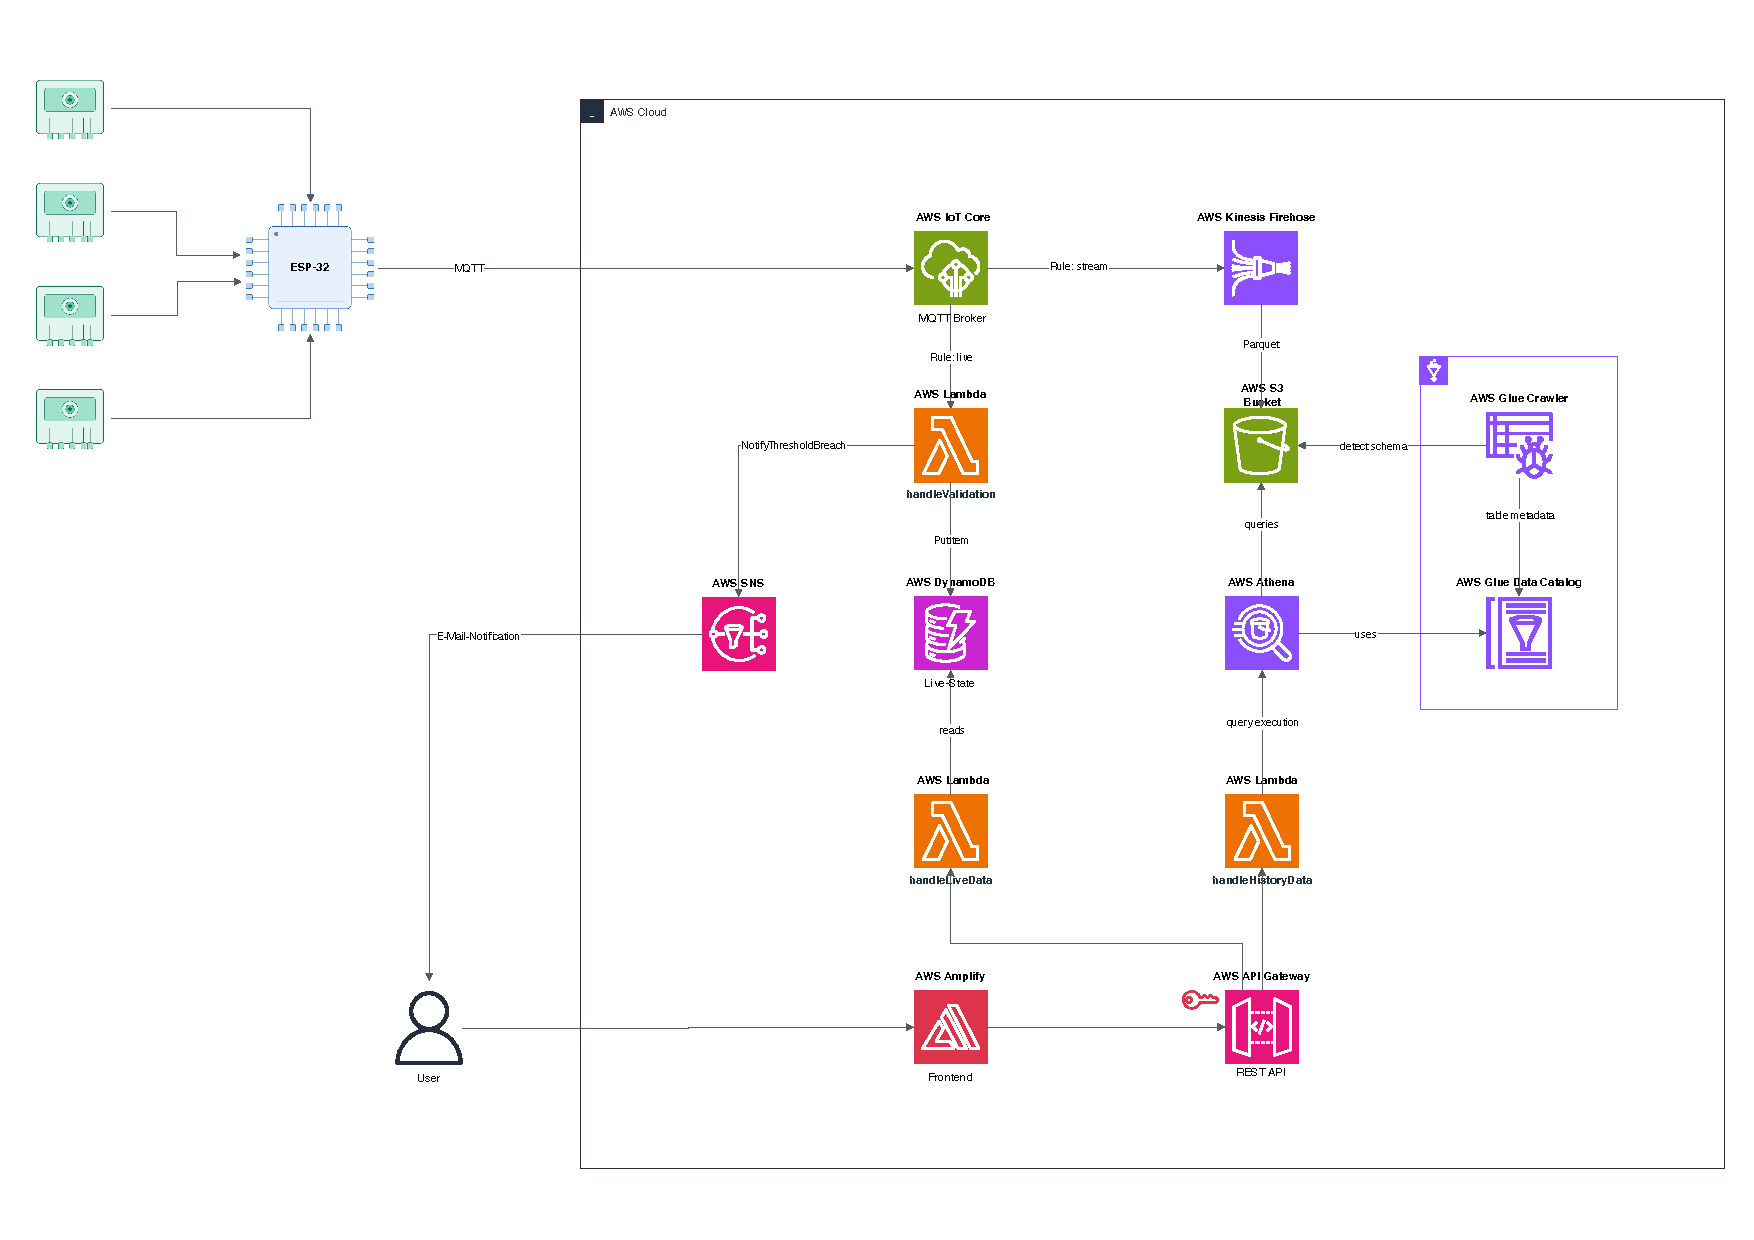
\includegraphics[width=\textwidth]{architecture.pdf}
  \caption{Cloud Processing Architecture}
  \label{fig:cloud-architecture}
\end{figure*}

% ----------------------------------------------------------------------
% Section 4 — Hardware
% ----------------------------------------------------------------------
\section{Hardware}\label{sec:hardware}
% TODO: remove section information
% Detailed description of the edge tier of the system.

The sensor node is the physical edge component of the Sensiq system
and is built around an ESP32 microcontroller hosting a set of
environmental sensors that cover temperature, humidity, ambient
light, air pressure, volatile organic compounds (VOCs), flame
radiation and high-temperature events. The following part of this
section first lists the individual hardware components and their
characteristics, then describes the firmware-level measurement
workflow (sensor initialization, periodic sampling, averaging and
MQTT publication), and finally documents the Steinhart--Hart
conversion used for the analog thermistor readings. The resulting
JSON payload sent to AWS IoT Core is described in
\cref{sec:mqtt_publication}.

\subsection*{Component Overview}\label{sec:component_overview}

The following hardware components are used in the sensor node:

\begin{description}
	\item[ESP32 NodeMCU board] Open-source development board carrying
	      the ESP-WROOM-32 module, breaking out 38~pins and providing a
	      CP2102 USB-to-serial bridge for programming and
	      power~\cite{esp32_berrybase}.
	\item[ESP-WROOM-32 module] Xtensa dual-core 32-bit LX6 CPU with up to
	      \SI{240}{\mega\hertz}, \SI{520}{\kilo\byte} SRAM and
	      \SI{4}{\mega\byte} SPI flash; integrated Wi-Fi
	      802.11\,b/g/n with up to \SI{150}{\mega\bit\per\second} and
	      Bluetooth; on-chip 12-bit SAR ADC (analog-to-digital converter) and
	      DAC (digital-to-analog converter). Supplied at
	      \SIrange{3.0}{3.6}{\volt}, operating range
	      \SIrange{-40}{85}{\celsius}~\cite{esp32_wroom_datasheet}.
	\item[DHT11] Single-wire digital temperature/humidity sensor;
	      range \SIrange{-20}{60}{\celsius} at \SI{\pm 2}{\celsius}
	      and \SIrange{5}{98}{\percent}~r.H.\ at
	      \SI{\pm 5}{\percent}~r.H.; sampling at
	      \SI{0.5}{\hertz}~\cite{dht11_asair}.
	\item[Joy-it KY-026 flame sensor] Detects flames in the IR band
	      \SIrange{760}{1100}{\nano\metre} with a \SI{60}{\degree}
	      detection cone up to \SI{100}{\centi\metre}. Provides an
	      inverted analog output (sampled by the ESP32 ADC) and a
	      potentiometer-adjustable digital threshold output for
	      event-driven triggering~\cite{ky026_joyit}.
	\item[Joy-it KY-028 thermistor] NTC temperature sensor covering
	      \SIrange{-55}{125}{\celsius} at \SI{\pm 0.5}{\celsius}.
	      Exposes an analog reading (ADC-limited rate) and a digital
	      over-temperature flag with adjustable
	      threshold~\cite{ky028_joyit}.
	\item[TSL2561 light sensor] Digital I\textsuperscript{2}C
	      ambient-light sensor with two photodiodes (visible and IR);
	      \SIrange{0.1}{40000}{\lux} at \SI{0.1}{\lux}
	      resolution~\cite{tsl2561_datasheet}.
	\item[Bosch BME680] Low-power I\textsuperscript{2}C/SPI sensor combining
	      temperature (\SI{\pm 1.0}{\celsius}), humidity
	      (\SI{\pm 3}{\percent}~r.H.), pressure
	      (\SI{\pm 0.6}{\hecto\pascal}) and a VOC gas channel
	      (\SIrange{2}{5}{\percent} accuracy for ethane, isoprene,
	      ethanol, acetone, CO) exposed as an IAQ index. Configurable
	      update rate up to \SI{1}{\hertz}; operating range
	      \SIrange{-40}{85}{\celsius} and
	      \SIrange{300}{1100}{\hecto\pascal}~\cite{bme680_bosch}.
	\item[Auxiliary switches] Two switches reserved for future work
	      on AI-based outlier detection with gathered training data
	      (see \cref{sec:summary}): one marks a reading as a labeled
	      training sample, the other flags a measurement as an
	      outlier.
\end{description}

The hardware design of the sensor node is presented from three
complementary perspectives.
\Cref{fig:hardware-circuit} shows the logical
circuit diagram made with the KiCAD software~\cite{kicad_software}and documents how the ESP32-DevKitC is wired to the
sensors, the two auxiliary switches and
the power supply, including the GPIO assignment of each signal
line.
\Cref{fig:hardware-pcb} in turn shows the resulting printed circuit board (PCB)
layout with the physical placement of the components, the routed
copper traces and the board outline intended for fabrication.
Both views are exported from the same KiCAD project and together
relate the firmware-level GPIO numbers used in the measurement
workflow to the corresponding physical pads on the planned PCB.
The PCB has not been manufactured yet, so the actual sensor node
shown in \cref{fig:hardware-picture} is built on a prototyping
board with the components manually placed and wired according to
the circuit diagram.

\begin{figure*}[!tb]
	\centering
	
\includegraphics[width=0.8\textwidth]{circuit_diagram_export_light.pdf}
	\caption{Circuit diagram of the sensor node, showing the
		logical wiring between the ESP32-DevKitC, sensors, the two
		auxiliary switches and the power supply, together with their
		respective GPIO assignments.}
	\label{fig:hardware-circuit}
\end{figure*}

\begin{figure}[htb]
	\centering
	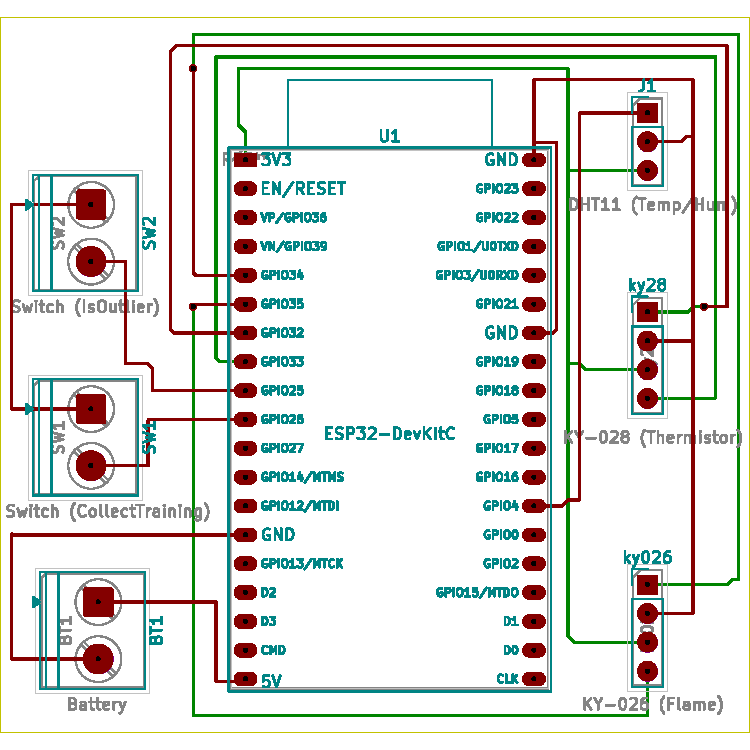
\includegraphics[width=0.95\linewidth]{pcb_pdf_export_light.pdf}
	\caption{PCB layout derived from the circuit diagram, showing
		the physical placement of the ESP32-DevKitC and the
		attached sensors, the routed copper traces and the board
		outline intended for fabrication.}
	\label{fig:hardware-pcb}
\end{figure}

\begin{figure}[htb]
	\centering
	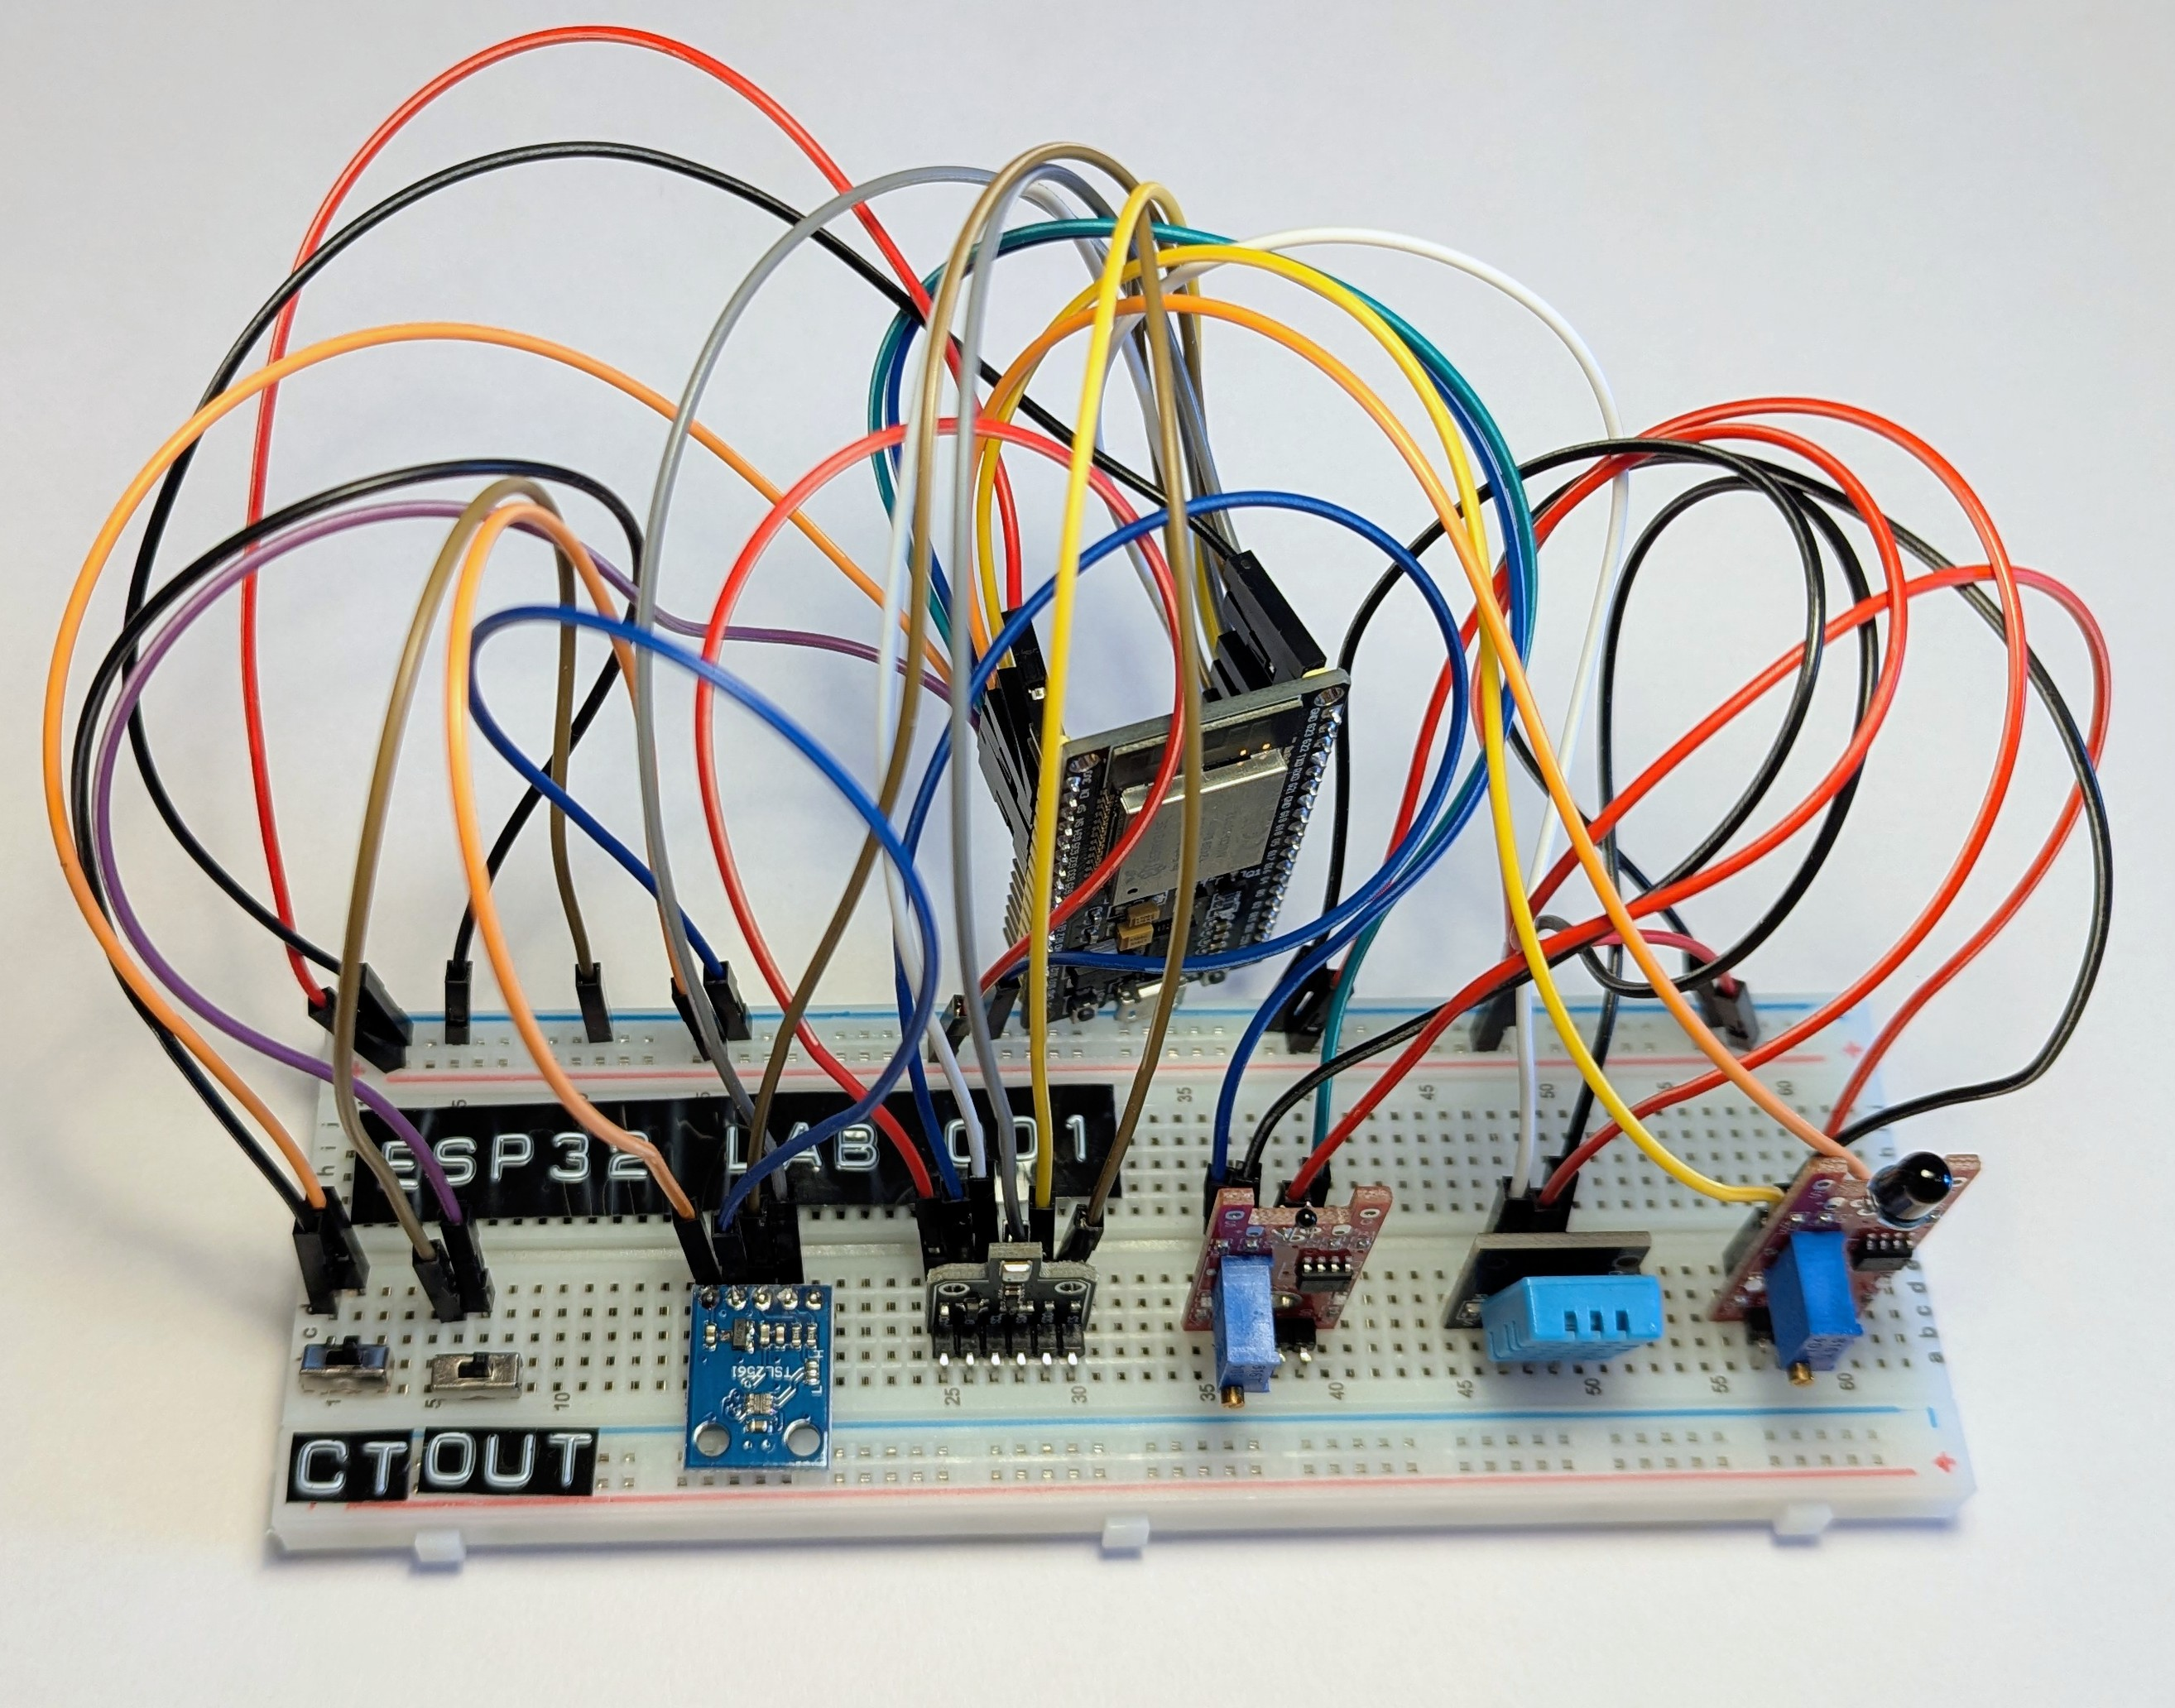
\includegraphics[width=0.95\linewidth]{hardware-picture.png}
	\caption{Real physical sensor node with the assembled sensors,
		the ESP32-DevKitC and the auxiliary switches.}
	\label{fig:hardware-picture}
\end{figure}

\subsection*{Measurement Workflow}\label{sec:measurement_workflow}
The firmware on the ESP32 follows a deterministic, two-phase
lifecycle written in Arduino C++~\cite{arduino_language_reference}:
a one-time \emph{startup} phase that prepares the
networking and sensing subsystems, followed by a continuously running
\emph{measurement loop}.

During startup the node performs the following steps in order:
\begin{enumerate}[leftmargin=*]
	\item Wi-Fi association: The node connects to a
	      configured local network using a pre-provisioned SSID and
	      password.
	\item Time synchronization: The internal clock is
	      synchronized with an NTP server. An accurate wall-clock
	      time is required both for meaningful measurement timestamps
	      and for the validation of TLS certificates during the
	      subsequent MQTT handshake.
	\item Sensor initialization: GPIO pin modes are set and
	      sensor-specific configuration (e.g. DHT11 configuration) is applied.
	\item MQTT setup: The MQTT client is configured (see~\cref{sec:mqtt_publication}).
\end{enumerate}

% small space for better readability
\medskip

Once startup is complete, the node enters its measurement loop:
\begin{itemize}[leftmargin=*]
	\item The MQTT connection is continuously validated and kept
	      alive; on disconnect, the client transparently reconnects.
	\item Every $t$ milliseconds a full sensor reading is taken
	      across all attached sensors with a default waiting period
	      of $t=\SI{1000}{\milli\second}$. Values smaller than one
	      second might not change much, as the sensors often have a
	      minimum sampling rate of \SI{1}{\hertz} or lower.
	\item After $n$ consecutive readings the buffered samples are
	      aggregated into a single record, serialized as JSON and
	      published to the configured MQTT topic. The standard
	      sample aggregation size is $n=5$, guaranteeing a balance
	      between responsiveness and noise reduction.
\end{itemize}
\medskip

Aggregation reduces sensor noise and the influence of isolated
outliers. It is performed per field according to its data type:
the most recent timestamp of the buffer is taken as the record
timestamp, numerical values (analog readings) are averaged
arithmetically, and digital boolean signals are decided by majority
voting over the buffered samples.

\medskip
\subsubsection*{Thermistor Conversion}

The KY-028 module exposes the thermistor as an analog voltage divider
that the ESP32 reads through its 12-bit ADC. The raw ADC value
$\mathrm{adc}\in[0,4095]$ is first converted to a resistance
$R$ assuming a sensor--internal \SI{10}{\kilo\ohm} pull-down resistor and a
\SI{3.3}{\volt} supply, and then to an absolute temperature using the
Steinhart--Hart equation~\cite{steinhart1968calibration}.
The equation models the resistance--temperature relationship of a
semiconductor thermistor as

\begin{equation}
	\frac{1}{T} = A + B \ln R + C (\ln R)^{3},
	\label{eq:steinhart_hart}
\end{equation}

where $T$ is the temperature in kelvin, $R$ is the thermistor
resistance in ohms at temperature $T$, and $A$, $B$ and $C$ are the
Steinhart--Hart coefficients characteristic of the specific
thermistor over the temperature range of interest. The firmware
uses the coefficients $A=1.129148\cdot 10^{-3}$,
$B=2.34125\cdot 10^{-4}$ and $C=8.76741\cdot 10^{-8}$, then converts
$T$ from kelvin to degrees Celsius before further using the value as
\texttt{thermistor\_temp}.

\subsection{MQTT Publication to AWS IoT Core}\label{sec:mqtt_publication}

The sensor node communicates with AWS IoT Core via the MQTT protocol over TLS.
% While an asynchronous MQTT client such as AsyncMQTT\_Generic \cite{asyncmqtt_generic_arduino}
% would theoretically offer non-blocking background execution and better performance
% during unstable connections, it currently lacks support for the required
% AWS IoT Core TLS certificates and is no longer maintained.
% Instead, the firmware utilizes the officially recommended MQTT library by
% Joel Gaehwiler~\cite{arduino_mqtt}, which provides only a synchronous API.

To establish a secure connection to the AWS IoT broker on port 8883,
the node requires the broker address and a set of cryptographic credentials.
The publicly available AWS Root CA certificate alongside the individual
device certificate and device private key are used for mutual TLS authentication.

% TODO: check if this got more values already.
\begin{lstlisting}[
    language=json, 
    float, 
    caption={Published JSON payload by the ESP32 sensor node via MQTT.}, 
    label={lst:data_model_json}]
{
    "running_time": 9881892,
    "timestamp": "2026-05-25T22:56:12Z",
    "device_id": "esp32-lab-001",
    "location": "Lab A, OTH Amberg-Weiden, 92224 Amberg, Germany",
    "dht_humidity": 61,
    "dht_temperature": 23.8,
    "dht_heat_index": 23.82809,
    "flame_analog": 0,
    "flame_digital": false,
    "thermistor_analog": 2005,
    "thermistor_digital": false,
    "thermistor_temp": 24.05634,
    "is_outlier": false,
    "collect_training": false
}
\end{lstlisting}

The MQTT topic structure is designed around a unique device identifier
(e.g., \texttt{esp32-lab-001}).
Data exchange uses three primary topics:
\texttt{sensiq/<identifier>/data} for publishing the aggregated sensor records,
\texttt{sensiq/<identifier>/test} for verifying connectivity, and
\texttt{sensiq/<identifier>/commands} reserved for receiving subsequent control commands.
\Cref{lst:data_model_json} shows an example of the JSON payload that the ESP32
node publishes to the data topic after each aggregation interval.

% ----------------------------------------------------------------------
% Section 5 — AWS Services
% ----------------------------------------------------------------------
\section{AWS Services}\label{sec:aws_services}
% TODO: remove section information
Detailed description of the cloud-side processing pipeline. Two
functional routes are exposed by the backend: a low-latency live
route and a long-term history route. Each is described in its own
subsection together with the AWS services it relies on.

\subsection{Live Route}\label{sec:live_route}
% TODO: remove section information
Path from IoT Core rule -> validation Lambda -> DynamoDB (latest
reading per device) -> API Gateway -> GET /live. Discuss latency
targets, payload shape, and error handling.

\subsection{History Route}\label{sec:history_route}
% TODO: remove section information
Path from IoT Core / validation Lambda -> S3 (Parquet, partitioned by
date) -> Glue catalogue -> Athena -> history Lambda -> API Gateway ->
GET /history. Discuss partitioning strategy, query patterns, and
expected query latency.

% ----------------------------------------------------------------------
% Section 6 — User Interaction
% ----------------------------------------------------------------------
\section{User Interaction}\label{sec:user_interaction}
The user has two ways of monitoring the environment´s state. An email notification can be
sent, when a value exceeds a certain threshold (\cref{sec:sns_notifications}), which allows for
passive, push-based monitoring. The second option is to actively monitor the web frontend (\cref{sec:frontend}),
which provides a detailed view of the live data and historical metrics.

\subsection{Email Notifications via SNS}\label{sec:sns_notifications}
The user gets ahold of critical environmental conditions by email notification.
Threshold evaluation is performed inside the \texttt{handleTransformValidate} Lambda function.
Each value is compared against a predefined threshold. Before each notification dispatch,
the Lambda Function checks against a DynamoDB~\cite{aws-dynamodb} Table \texttt{emailDB}, which holds the latest
email and the reason for its dispatch. An email is sent only if the entry is at least 300 seconds old. AWS SNS~\cite{aws-sns}
handles notifications, and delivers an email to predefined addresses, which are currently
manually set. The user receives a detailed overview over the current state of the
device and the metric that caused the alarm.

\subsection{Web Frontend}\label{sec:frontend}
Describe the React-based dashboard hosted on AWS Amplify: live tiles,
historical charts, sensor status indicators, and authentication via
AWS Cognito. Include a screenshot or mock-up
(see template: figure*).

% ----------------------------------------------------------------------
% Section 7 — Evaluation
% Rationale: Testability and cost are assessment results rather than
% design decisions; grouping them in a dedicated Evaluation section
% separates "what was built" from "how it was assessed".
% ----------------------------------------------------------------------
\section{Evaluation}\label{sec:evaluation}

\subsection{Testability}\label{sec:testability}
% TODO: remove section information
% Discuss per-service testability: Lambda unit tests (SAM CLI), local
% emulation of DynamoDB / S3 / API Gateway, limitations for IoT Core
% (Device Advisor only), and the role of LocalStack for higher-level
% integration tests.

\subsubsection{Sensor Node Firmware}
The testability of the sensor node, built around the ESP32 microcontroller
(see \cref{sec:hardware}), presents specific challenges due to its embedded nature.
Unit testing of the firmware is implemented using the AUnit
framework~\cite{aunit_testing_arduino}, which is structured such that either the test suite or the main
measurement loop executes, preventing interference between testing and regular operation.

Unit tests are implemented for isolated modules such as the sensor readings,
sensor data aggregation, Wi-Fi connection, basic MQTT connection and
configuration settings. However, exhaustively testing the MQTT
publication functionality described in \cref{sec:mqtt_publication} via unit tests is
not feasible without extensive mocking. Since such mocking would deviate significantly
from real-world behavior, and the underlying MQTT library is already well-tested
and established in the community, complex local test implementations for MQTT were omitted.

Instead, the hardware node employs a direct feedback mechanism for connectivity
validation during its real-world measurement workflow. Upon successfully
establishing a connection to the MQTT broker, the node subscribes to the test
topic to verify the connection's health, ensuring the publish functionality
operates correctly in the physical environment.

\subsection{Cost Estimation}\label{sec:cost_estimation}
% TODO: remove section information
% Present the monthly operating-cost estimate per device under realistic
% assumptions (users, active hours, message volume). Compare Free Tier
% and Post Free Tier costs across all involved AWS services.
% Template available at end of document: tab:aws-costs.

\subsubsection{Hardware Cost}
The one-time hardware cost per sensor node is based on the components used for prototyping.
A breakdown of the individual component costs is presented in \cref{tab:hw-costs}.

\begin{table}[htb]
	\centering
	\caption{Hardware Cost per Sensor Node}
	\label{tab:hw-costs}
	\small
	\begin{tabularx}{0.7\linewidth}{>{\raggedright\arraybackslash}X r r}
		\toprule
		\textbf{Component}         & \textbf{Unit Cost}     \\
		\midrule
		ESP32-DevKitC              & 8\,€                   \\
		Bosch BME680               & 18\,€                  \\
		TSL2561 Light Sensor       & 5\,€                   \\
		DHT11 Sensor               & 3\,€                   \\
		Joy-it KY-026 Flame Sensor & 3\,€                   \\
		Joy-it KY-028 Thermistor   & 3\,€                   \\
		Prototyping equipment      & \(\sim\)3\,€           \\
		\midrule
		\textbf{Total}             & \textbf{\(\sim\)43\,€} \\
		\bottomrule
	\end{tabularx}
\end{table}


% ----------------------------------------------------------------------
% Section 8 — Summary and Future Work
% ----------------------------------------------------------------------
\section{Summary and Future Work}\label{sec:summary}

% \subsection*{Summary}
Sensiq provides a scalable, end-to-end IoT solution for continuous laboratory environment monitoring.
By combining a low-cost ESP32 sensor platform with a serverless AWS backend and a React dashboard,
the system successfully delivers both low-latency alerting and robust historical analysis.
It reliably monitors critical metrics including temperature, humidity, and air quality while
maintaining a highly efficient operational footprint of under three U.S. dollars per node monthly.

% \subsection*{Future Work}
As detailed in the evaluation (\cref{sec:discussion}), future development prioritizes security,
analytical maturity, and deployment flexibility. Planned operational improvements include
migrating to AWS Cognito for robust authentication and enabling dynamic, per-device configuration
of warning thresholds and notification recipients directly within the frontend.
On the hardware level, integrating optimizing power
consumption via deep-sleep configurations will broaden deployment capabilities.
Lastly, introducing machine learning models will enhance the system with real-time outlier
detection in the live data stream, providing preemptive anomaly alerts that overcome the limitations
of static, threshold-based evaluation.

% ======== References =========
\sloppy
\printbibliography[notcategory=selfref]

\end{document}

% ======================================================================
% TEMPLATES
% The following snippets are preserved as reference templates for tables,
% figures, listings, and other recurring constructs. They are kept here
% (after \end{document}) so they are not compiled but remain available
% for copy-and-paste into the new section files.
% ======================================================================

% ---------- Template: Comparison Table (tabularx, booktabs) ------------
% \begin{table}[htb]
%     \centering
%     \caption{Comparative Analysis of Monitoring Architectures}
%     \label{tab:comparison}
%     \small
%     \begin{tabularx}{\linewidth}{>{\raggedright\arraybackslash}X c c c}
%         \toprule
%         \textbf{Feature} & \textbf{Col A} & \textbf{Col B} & \textbf{Col C} \\
%         \midrule
%         Row 1 & Yes & Yes & Yes \\
%         Row 2 & Limited & High & High \\
%         \midrule
%         \textbf{Suitability} & \textbf{Medium} & \textbf{Medium} & \textbf{High} \\
%         \bottomrule
%     \end{tabularx}
% \end{table}

% ---------- Template: MoSCoW-style Table --------------------------------
% \begin{table}[!h]
%     \centering
%     \caption{MoSCoW Prioritization of User Stories}
%     \label{tab:moscow_prioritization}
%     \begin{tabularx}{0.9\linewidth}{>{\raggedright\arraybackslash}p{2.8cm} >{\raggedright\arraybackslash}X}
%         \toprule
%         \textbf{Category} & \textbf{User Stories} \\
%         \midrule
%         Must Have   & \hyperref[sec:us_01]{Story A}, \hyperref[sec:us_02]{Story B} \\
%         Should Have & \hyperref[sec:us_03]{Story C} \\
%         Could Have  & \hyperref[sec:us_04]{Story D} \\
%         Won't Have  & \hyperref[sec:us_05]{Story E} \\
%         \bottomrule
%     \end{tabularx}
% \end{table}

% ---------- Template: Wide Cost-Estimation Table (table*) ---------------
% \begin{table*}[!htb]
%     \centering
%     \caption{Cost Estimation for AWS Services}
%     \label{tab:aws-costs}
%     \begin{tabularx}{0.8\textwidth}{>{\raggedright\arraybackslash}l >{\raggedright\arraybackslash}l >{\raggedright\arraybackslash}r >{\raggedright\arraybackslash}r}
%         \toprule
%         \textbf{Service Details} & \textbf{Usage/Quantity} & \textbf{Free Tier} & \textbf{Post Free Tier} \\
%         \midrule
%         Service A & Usage A & \$0.00 & \(\sim\)\$0.06 \\
%         Service B & Usage B & \(\sim\)\$0.01 & \(\sim\)\$0.08 \\
%         \midrule
%         \textbf{Total} & & \textbf{\(\sim\)\$0.46} & \textbf{\(\sim\)\$0.73} \\
%         \bottomrule
%     \end{tabularx}
% \end{table*}

% ---------- Template: Full-width Figure (figure*) -----------------------
% \begin{figure*}[!tb]
%   \centering
%   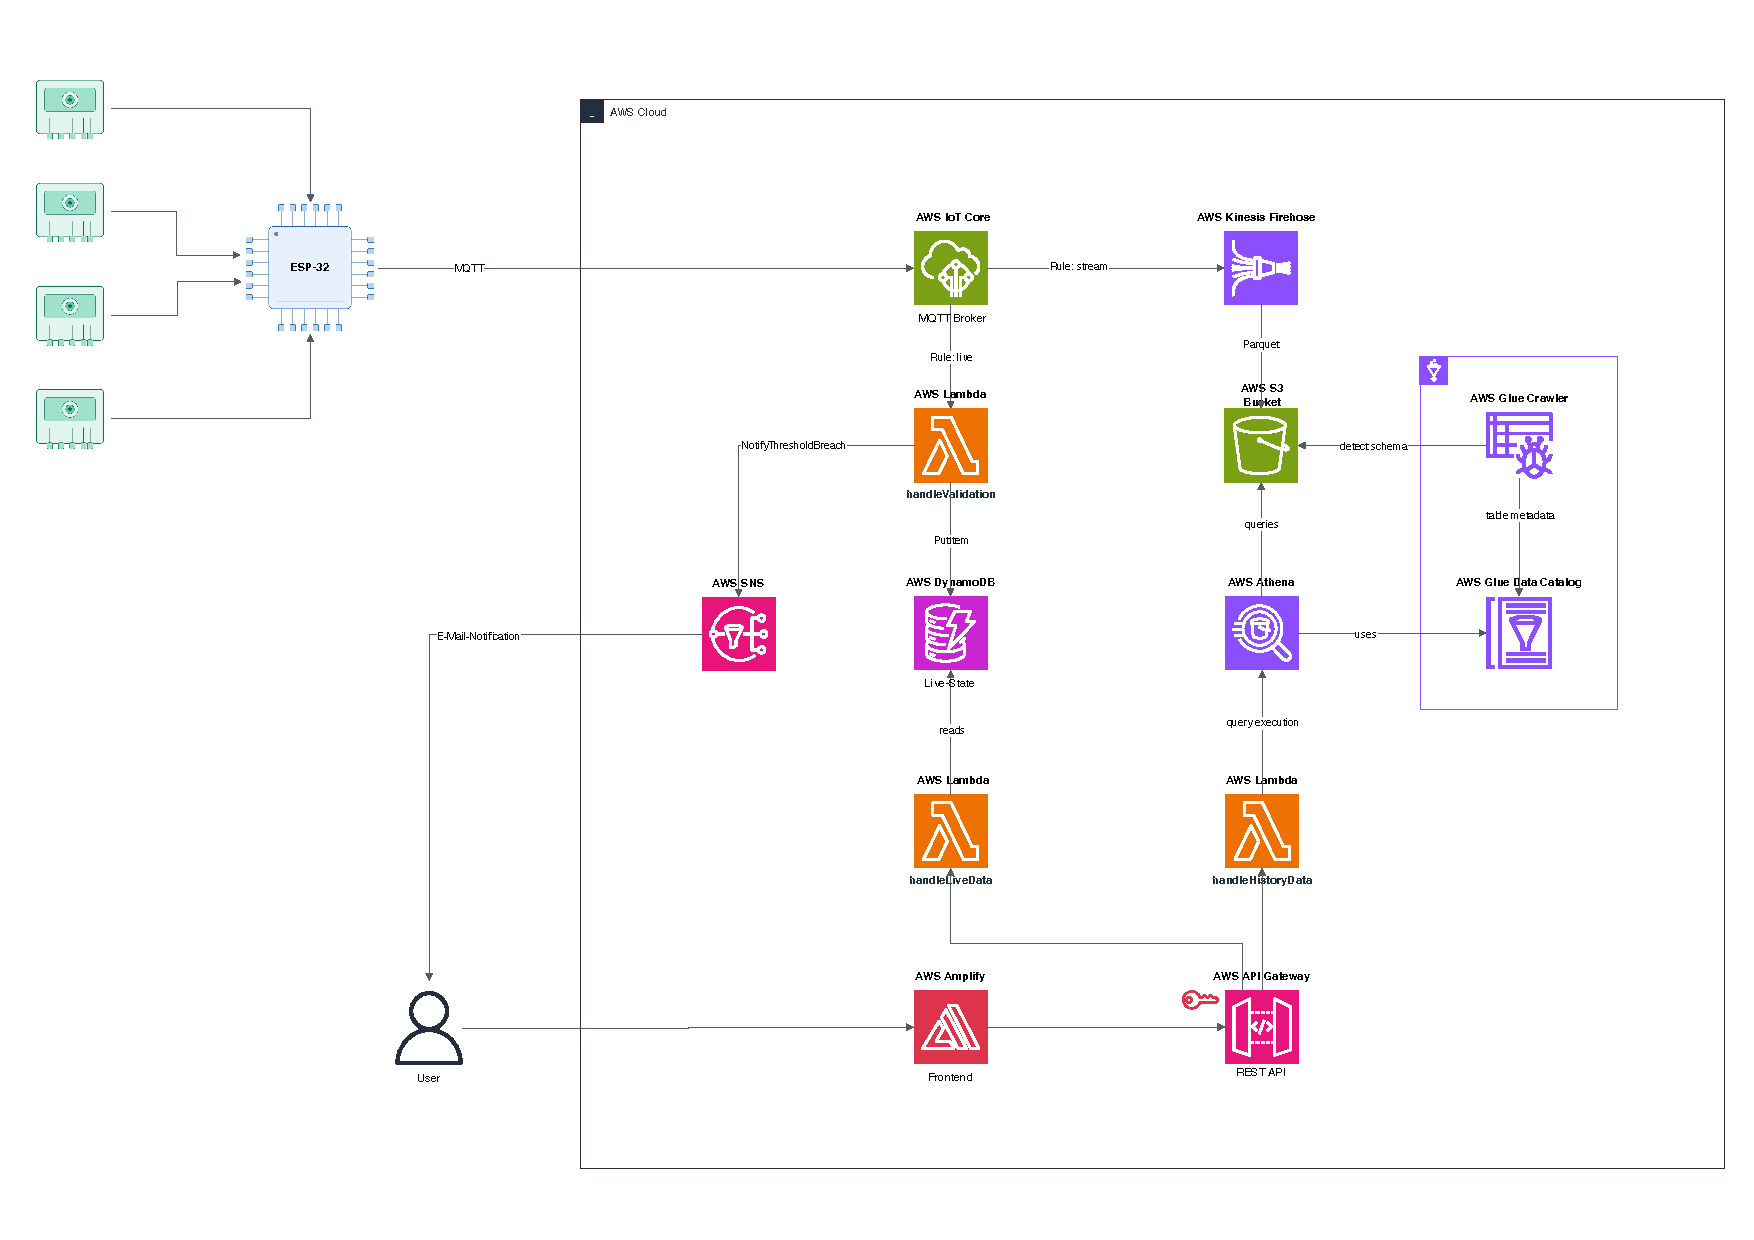
\includegraphics[width=\textwidth]{architecture.pdf}
%   \caption{Cloud Processing Architecture}
%   \label{fig:cloud-architecture}
% \end{figure*}

% ---------- Template: JSON Code Listing ---------------------------------
% \begin{lstlisting}[language=json, float, caption={Example JSON data model.}, label={lst:data_model_json}]
% {
%   "deviceId": "esp32-lab-01",
%   "measurements": {
%     "dht11_temperature": { "value": 20, "unit": "degree C" }
%   }
% }
% \end{lstlisting}

% ---------- Template: Description List (Personas etc.) ------------------
% \begin{description}
%     \item[Persona Name] Short description of role, goals, and interests.
% \end{description}

% ---------- Template: Itemized Acceptance Criteria ----------------------
% \begin{itemize}
%     \item Criterion 1: measurable expectation with input/output.
%     \item Criterion 2: timing requirement (e.g., update within 10\,s).
% \end{itemize}

% ---------- Template: Block Quote (User Story) --------------------------
% \begin{quote}
%     \textit{As <Persona>, I want <goal>, so that <benefit>.}
% \end{quote}
